%Appendix Appendix Appendix
\begin{appendices}

\section{Numerically stable tensor inner product (in log-domain)}


\label{sec:appendix_tmul}
The operation of computing ratios of probabilities is typically unstable, especially if the probabilities have small values. In order to average over a large number of importance samples in log-domain, we need a numerically stable method. If we compute    
\begin{equation*}
    e^{Z_{ik}} = \sum_j e^{X_{ij}}e^{Y_{jk}},
\end{equation*}
in order to get
\begin{equation*}
    Z_{ik} = \log \sum_j e^{X_{ij}}e^{Y_{jk}},
\end{equation*}
very large or small values of $X_{ij}$ and (or) $Y_{jk}$ could lead to numerical instability. To circumvent this issue, we subtract the largest values along $j$ before computing the sum. Then, to ensure the correctness of our marginal log-likelihoods, we add these values back as follows
\begin{equation*}
    Z_{ik} = \log \sum_j e^{X_{ij} - \text{max}_j({X_{ij})}}e^{Y_{jk} - \text{max}_j(Y_{jk})} + \text{max}_j({X_{ij}) + \text{max}_j}(Y_{jk}) 
\end{equation*}

\section{TMC Architecture}
\label{sec:appendix_tmc_arch}
Here we present a graphical overview of the model architecture we used for the TMC.
\begin{figure}[h]
\begin{center}
\makebox[\textwidth][c]{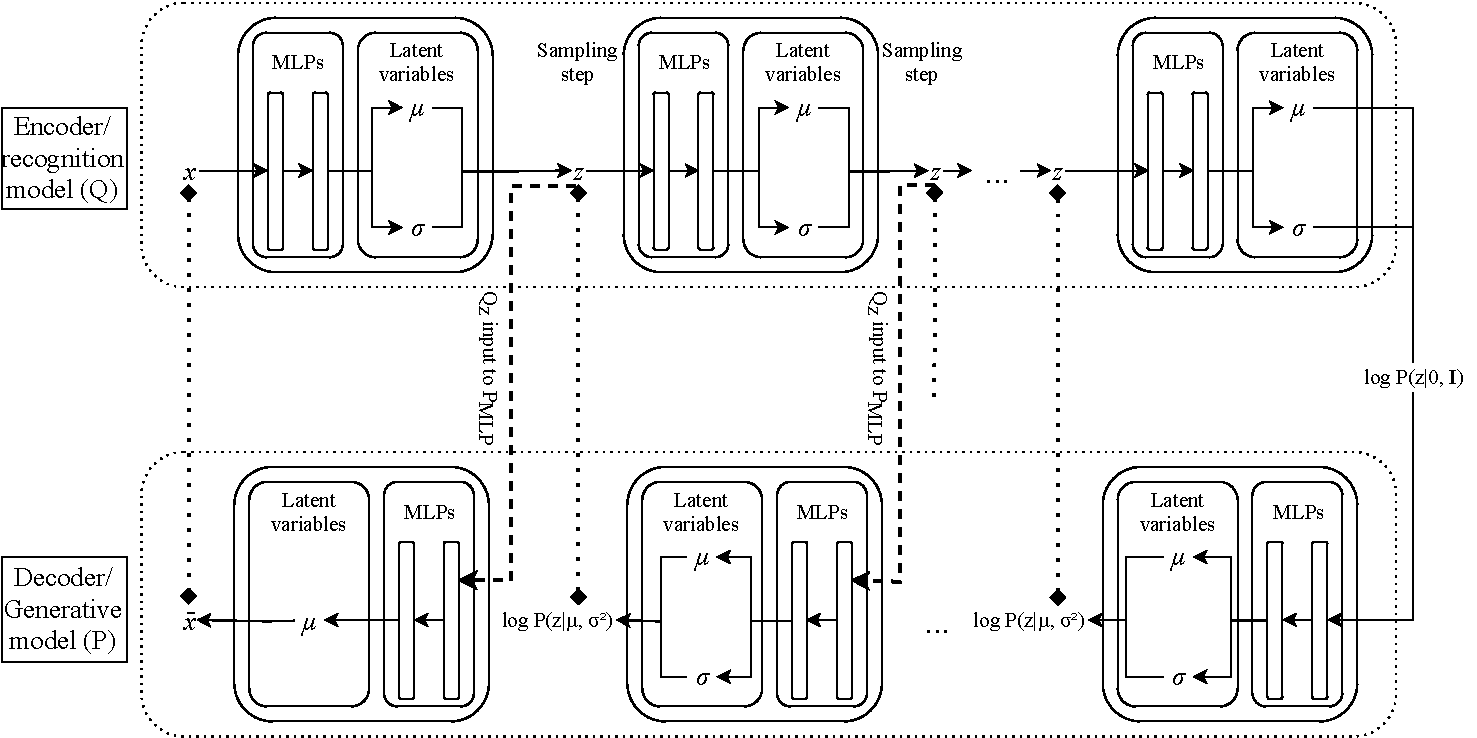
\includegraphics[width=1.25\textwidth]{Figures/tmc.pdf}}%
\end{center}
\caption{TMC architecture as textually presented (\cite{tmc}). The final stochastic layer in the generative model assumes a Bernoulli distribution, why only the mean is computed in the corresponding MLP.}
\label{fig:tmc_layout}
\end{figure}


\section{Reconstructions}
\label{sec:app_rec}
Below we display the reconstructions for the small IWAE (left) and small TMC (right) models, given an observation (sample) from the MNIST test set. In both figures, the far left column shows the input test samples (original), and the remaining columns the reconstructions. 

\begin{figure*}[th!]
    \centering
    \begin{subfigure}[t]{0.5\textwidth}
    \hspace*{-2cm}
        \centering
        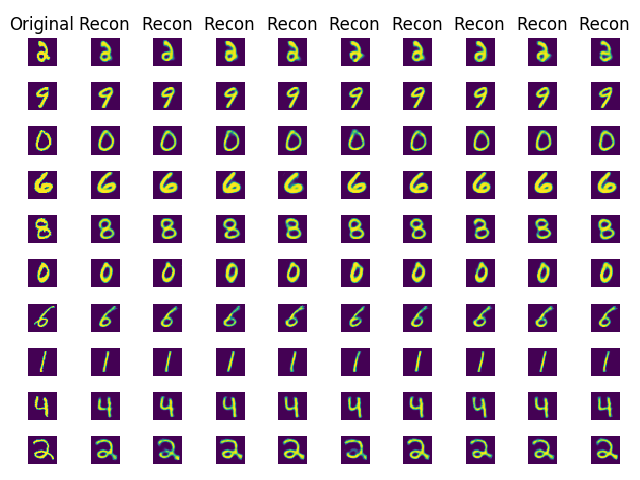
\includegraphics[height=6cm]{Figures/IWAE_recon_small.png}
    \end{subfigure}%
    ~ 
    \begin{subfigure}[t]{0.5\textwidth}
        \centering
        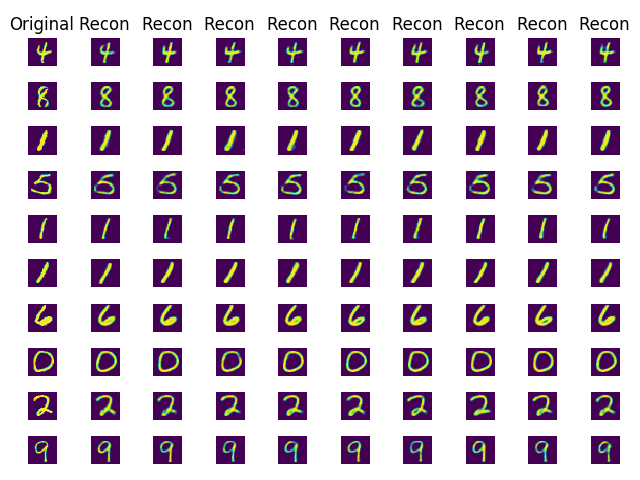
\includegraphics[height=6cm]{Figures/TMC_recon_small.png}
    \end{subfigure}
    \caption{Reconstructions from the small IWAE (left) and TMC (right) models, after 1200 epochs of training.}
    \label{fig:reconstructions}
\end{figure*}

\section{Clustering}
\label{sec:clusters}
We compared the clustering abilities for the IWAE versus the TMC algorithms, given a two-dimensional latent space (the latent space farthest from the data). In this experiment, there were two stochastic layers in the recognition model with dimensions 50 and 2 (deterministic layers [100, 100] and [100, 100] for the two MLPs). To obtain these data points, we averaged over $K$ for every latent. It is apparent from Fig. \ref{fig:clusters} that the TMC offers a richer latent space than the IWAE, for this specific architecture. For instance, note how the digit nine's representation (view color bar) is not mixing as much, for the TMC (right), with its neighboring clusters as is the case for the IWAE (left).
\begin{figure*}[h!]
    \centering
    \begin{subfigure}[t]{0.5\textwidth}
    \hspace*{-2cm}
        \centering
        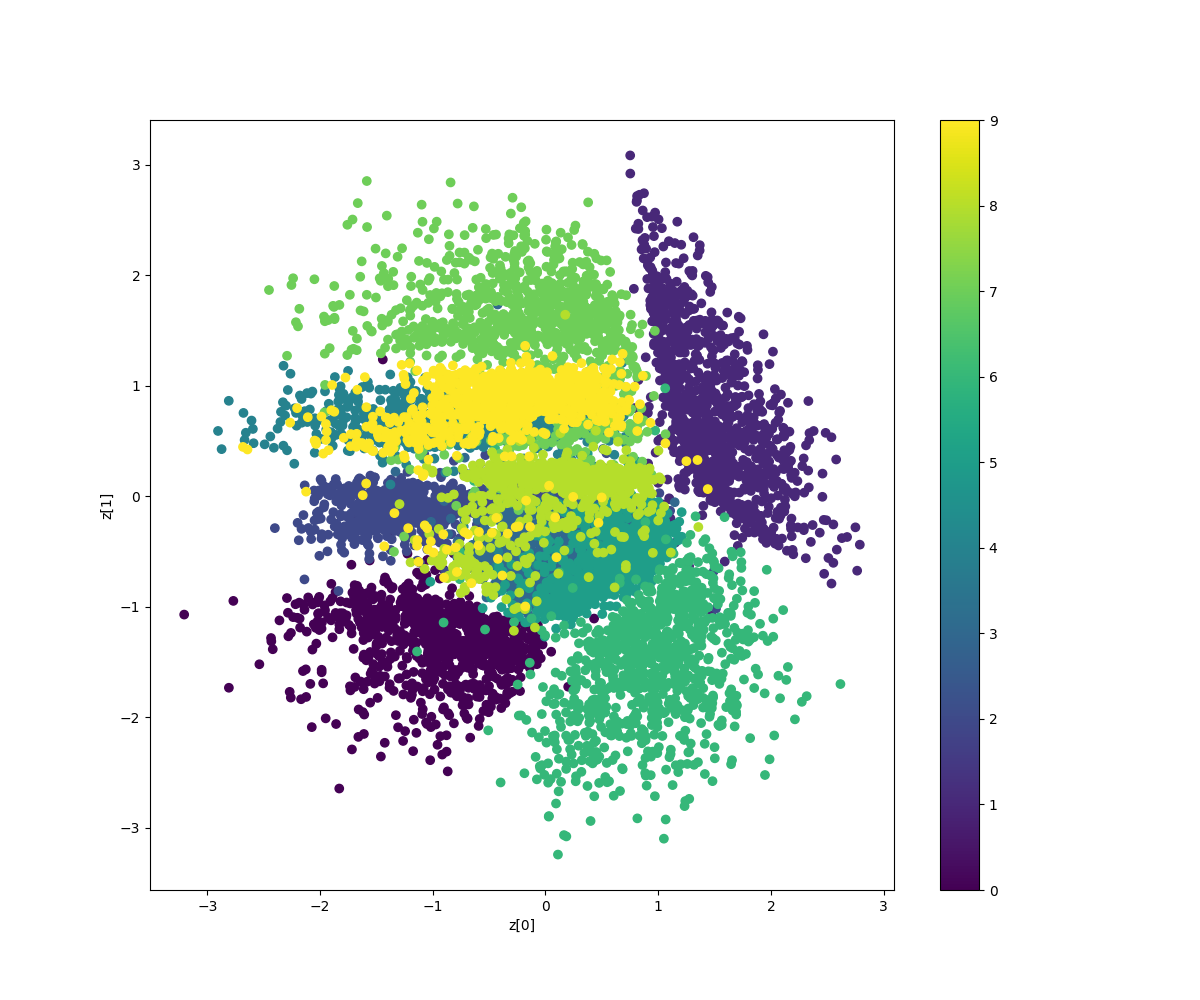
\includegraphics[height=8cm]{Figures/Scatter_plot_iwae.png}
    \end{subfigure}%
    ~ 
    \begin{subfigure}[t]{0.5\textwidth}
        \centering
        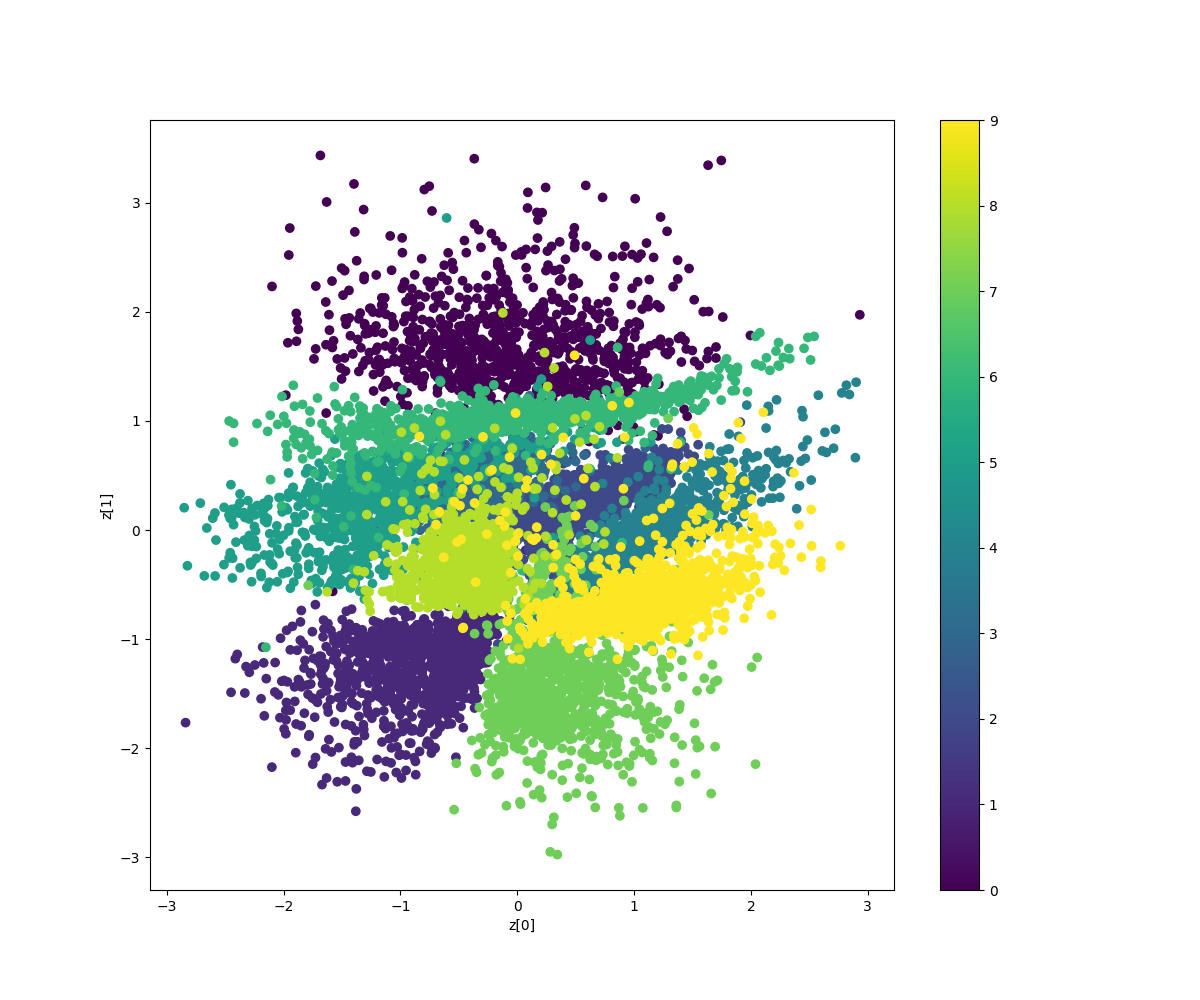
\includegraphics[height=8cm]{Figures/Scatter_plot_tmc.png}
    \end{subfigure}
    \caption{Clusters in a two dimensional latent space by the IWAE (left) and TMC (right), after 700 epochs of training and the special architecture mentioned in Appendix \ref{sec:clusters}. Best viewed in color. }
    \label{fig:clusters}
\end{figure*}
\end{appendices}